\documentclass{article}
\usepackage[utf8]{inputenc}
\usepackage{graphicx}
\usepackage{verbatim}
\usepackage{listings}
\usepackage{amsmath}
\usepackage{tikz}
\usepackage{rotating}
\usetikzlibrary{positioning}
\usepackage{bussproofs}
\usepackage{turnstile}
\usepackage{stmaryrd}
\usepackage{caption}
\usepackage{subcaption}

\usepackage{cancel}
\newcommand{\lnec}{\Box}

\usepackage[edges]{forest}
\usepackage{amssymb}
\usepackage{comment}

\newcommand\mymapsto{\mathrel{\ooalign{$\rightarrow$\cr%
    \kern-.15ex\raise.275ex\hbox{\scalebox{1}[0.522]{$\mid$}}\cr}}}
\definecolor {processblue}{cmyk}{0.96,0,0,0}

\title{DM872 assignment 1}
\author{sagra16 \\(Valdemar Grange - 081097-2033) }
\date{May 2020}

\begin{document}

    \maketitle

    \section{Introduction}
    In this report I will document my attempt at creating a good schedule for events.
    These events are derived from SDU IMADA/NAT events and the model is then scored in $4$ different ways.
    I have used \texttt{gurobi} as the solver for my MILP model, and a feasible solution is found given enough time.

    \section{The model}
    The model was to have some different hard-constraints as listed in the project description.
    The objective function will be discussed at the end once all the parts have been discussed.
    I have introduced some new sets to help develop this model which have reduced the set-up time of the model tremendously (about a 20x speed increase) and smaller but noticeable solve time.
    The first of these are a set $B_r$ which is a collection of busy times for a given room $B = \{ B_r \subset P \,|\, r \in R \}$, note that this includes the banned slots from \texttt{timeslots.json} and busy from \texttt{rooms.json}.
    I will also use $E_w$ to denote all the events for week $w \in P$.
    This has an enormous impact on the time spent creating constraints, as the amount of events for a specific week is substantially smaller than the whole set of events.
    Further notation will be introduced it appears.
    Finally I have chosen that my "allocation" or "activation" variable $x$ is indexed by event $e \in E$, room $r \in R$ and time $p \in P$.
    \subsection{Hard constraints}
    \subsubsection{}
    First I have the simple constraints that $x_{e,r,p}$ is boolean and all events must be scheduled.
    Additionally I introduce the function $week: E \rightarrow \mathbb{N}$ which evaluate the scheduled week for an event (from the data).
    \[x_{erp} \in \{0, 1\}\]
    \[\sum_{(h,d,w) \in P, r \in R} x_{e,r,(h,d,week(e))} = 1, \forall e \in E\]
    The constraint states that every event must be scheduled exactly once.
    \subsubsection{}
    Next is the constraint that will ensure that no two events will ever overlap in the same room.
    \[\sum_{e \in E_w} \, \sum^h_{i=max(0, h - \ell(e) + 1)} x_{e,r,(i,d,w)} \leq 1, \, \forall (h,d,w) \in P, \, \forall r \in R\]
    Here I make use of a new and unfamiliar sum $\sum^h_{i=max(0, h - \ell(e) + 1)}$.
    This sum ensures that for some time $(h,d,w)$ and all events for the week $e$, the amount of "active" events within the time-range $\{ h - \ell(e) + 1 .. h \}$ cannot be more than $1$.
    In other words, at some point this $(h,d,w)$ will be at the last scheduled time for an event $e$, at that moment and $h - \ell(e) + 1$ steps back, only one event must be scheduled (namely the event $e$).
    We will see more of this time-range sum.
    \subsubsection{}
    This constraint states that a teacher may not teach two classes at the same time.
    Or more specifically, no more than one room may ever be occupied by a class that requires the same teacher within the entire time-frame of a lecture.
    I will additionally denote teacher events by the week they are scheduled in by $de \in D_w$.
    \[\sum_{e \in de} \, \sum_{r \in R} \, \sum^h_{i=max(0, h - \ell(e) + 1)} x_{e,r,(i,d,w)} \leq 1 , \, \forall de \in D_w, \, \forall (h,d,w) \in P,\]
    \subsubsection{}
    Here I simply ensure that no events are scheduled to run during banned periods.
    Note that I use the time-range sum here, since a event potentially could start before a banned time and range over it.
    \[\sum^h_{i=max(0, h - \ell(e) + 1)}  x_{e,r,(i,d,w)} = 0 ,\, \forall e \in E_w ,\, \forall (h,d,w) \in B_r ,\, \forall r \in R\]
    \subsubsection{}
    Now I introduce the modelling of the precedence graph, which should model the precedence within a week.
    I model this by using the "activation" day.
    If the class is allocated in day $3$ its binary value will be $1$, thus the allocated day will be $1*3$.
    The difference between the in-arc vertex's day in $e_1$ and the current day in $e_2$ must be at least $1$ (in favor of the preceding vertex being larger).
    \[\hspace*{-1cm}\left(\sum_{r \in R} \, \sum_{(h,d,w) \in P} x_{e_2,r,(h,d,week(e_2)} * d \right) - \left(\sum_{r \in R} \, \sum_{(h,d,w) \in P} x_{e_1,r,(h,d,week(e_1)} * d \right) \geq 1, \, \forall e_1e_2 \in A, \, \forall e_2 \in E\]
    \subsubsection{}
    The constraint for "there is at most one event per course per day for each student", needs an introduction of a new set $H_{d,w}$.
    $H_{d,w}$ is simply a set of hours for some $d,w \in P$.
    Note that any combination of $h,d,w$ are implied as unique combinations of the original set.
    Moreover the inclusion of the course has warranted two new additions, $C$ which is the set of courses and $Q_{c_w}$ which is the set of student events for some course and week.
    $$\sum_{r \in R} \sum_{e \in q} \sum_{h' \in H_{d,w}} x_{e,r,(h',d,w)} \leq 1, \, \forall q \in Q_{c_w}, \, \forall c \in C , \, \forall (d,w) \in P$$
    \subsubsection{}
    The final hard-constraint states that no event may exceed the last hour.
    This is modelled by introducing $final_{d,w}$ which is the final hour for a given day and week (or also expressed as $max(H_{d,w})$).
    I use the time-range sum again, but here I only use the $final_{d,w}$ as my $h$.
    The constraint will ensure that no lessons are scheduled such that they exceed the final hour of the day.
    $$\sum^{final_{d,w}}_{i=max(0, final_{d,w} - \ell(e) + 1)} x_{e,r,(i,d,w)} = 0, \, \forall e \in E_w , \, \forall (d,w) \in P , \, \forall r \in R$$
    \subsection{Objectives}
    In the objectives I can give value to different assignments and formulate what better solutions are.
    \subsubsection{}
    Discomfort is minimized in regard to bad slots.
    Let $O$ be the set of $c_p$ where $p \in P$ and $c \in \mathbb{N}$, $c$ being an arbitrary weight of how "bad" a timeslot is.
    The minimum value this $c$ may take is $1$.
    $$\alpha = \sum_{(h,d,w) \in P} \, \sum_{e \in E_w} \, \sum_{r \in R} \, \left( \sum^h_{i=max(0, h - \ell(e) + 1)} x_{e,r,(i,d,w)} \right) * c_{h,d,w}$$
    In practice I have chosen the following values:
    \begin{center}
        \begin{tabular}{|c | c | c |}
            \hline
            Time & Day(s) & $c$ \\ [0.5ex]
            \hline
            8 & Mon-Fri &  5  \\
            \hline
            16 & Mon-Thu & 3  \\
            \hline
            17 & Mon-Thu & 4  \\
            \hline
            15, 16, 17 & Fri & 6  \\ [1ex]
            \hline
        \end{tabular}
    \end{center}
    \subsubsection{}
    The number of events per day should be as low as possible.
    I find the maximum lectures $ml$ of any one day for any one teacher, this should be minimized.
    An average case minimization is harder to formulate because of the requirement of linearity (a sum of squares technique would be a nice alternative).
    \[ml \geq \sum_{e \in de} \, \sum_{h' \in H_{d,w}} \, \sum_{r \in R} x_{e,r,(h',d,w)}, \, \forall de \in D_w, \, \forall (d,w) \in P\]
    Since the solver is free to assign anything to $ml$, it will assign the smallest possible value that satisfies the constraint, eg the maximum of the right hand side of $\geq$.
    \subsubsection{}
    Like the previous constraint, an average case analysis is difficult, so I settle with the above strategy.
    I employ the same strategy as above; minimization of the maximum amount of concurrent events for a student for any given time.
    \[\beta \geq \sum_{e \in q} \sum_{r \in R} \, \sum^h_{i=max(0, h - \ell(e) + 1)} x_{e,r,(i,d,w)}, \, \forall q \in Q_w , \, \forall (h,d,w) \in P \]
    \subsubsection{}
    Finally the most difficult constraint to formulate, weekly stability.
    Weekly stability in regard to events being scheduled the same day every week, I find the day where the maximum amount of events take place, I then maximize this.
    A course is $E_c = \{e \in E | e \in C_c \}$
    \[\Delta_{c,d} =  \sum_{(h,w) \in P} \, \sum_{e \in E_{c_w}} \,\sum_{r \in R}  x_{e,r,(h,d,w)}, \, \forall d \in P, \, \forall c \in C\]
    Assuming our objective is the following:
    \[\delta_c \geq \Delta_{c,d} , \, \forall d \in P\]
    There is actually a problem here; $\delta_c$ can take \textbf{any} value in $\mathbb{N}$, so maximizing this would instantly result in $\delta_c = max(\mathbb{N}) , \, \forall c \in C$.
    \\\\
    I can get around this by using activation variables $y_{c,d}$ and big $M$ (which I simply assign to $|E|$ since a there can be at minimum $1$ course with length $E$).
    The strategy is to have a $z_c$ take the maximum value of $\Delta_{c,d}, \, \forall d \in P$.
    I can achieve this by "offsetting" a $\Delta_{c,d}$ by $\Delta_{c,d} + M y_{c,d}$ resulting in a value much larger than any value $\Delta_{c,d}$ can take, I then ensure that the solver must \textbf{only} assign $|\{d \in P\}| - 1$ values of $y_{c,d} = 1$, result in the solver picking the largest $\Delta_{c,d}$ as the "non scaled".
    $z_c \leq \Delta_{c,d} + M y_{c,d}$.
    Asking the solver to maximize this will result in the solver "picking" a $y_{c,d} = 0$ that results in the maximum of $z_c$ which of course will be $z_c = max(\{\Delta_{c,d} | d \in P\})$.
    \begin{gather*}
        y_{c,d} \in \{0, 1\}\\
        M = |E|\\
        z_c \in \mathbb{N}\\
        \sum_{d \in P} y_{c,d} = |\{d \in P\}| - 1 , \, \forall c \in C\\
        z_c \leq \Delta_{c,d} + M y_{c,d} , \, \forall d \in P , \, \forall c \in C\\
    \end{gather*}
    In practice we can instead use:
    \[
        \sum_{d \in P} y_{c,d} \leq |\{d \in P\}| - 1 , \, \forall c \in C\\
    \]
    Since largest $y_{c,d}$ will be deactivated.
    I do this because $\geq$ and $\leq$ reduce the problem complexity.\\
    Note the importance of restricting events to courses and that we invert the expression to make it a minimization problem instead of maximization.

    \subsection{Putting it together}
    Note that I split the precedence graph up into a variable for readability.
    \begin{equation*}
        \hspace{-1cm}
        \begin{array}{ll@{}ll}
            \text{minimize}  & \displaystyle\alpha + ml + \beta - \sum_{c \in C} z_c &\\
            \text{subject to}& \displaystyle\sum_{(h,d,w) \in P, r \in R} x_{e,r,(h,d,week(e))} = 1,  & \, \forall e \in E\\
            & \displaystyle\sum_{e \in E_w} \, \sum^h_{i=max(0, h - \ell(e) + 1)} x_{e,r,(i,d,w)} \leq 1, & \, \forall (h,d,w) \in P, \, \forall r \in R\\
            & \displaystyle\sum_{e \in de} \, \sum_{r \in R} \, \sum^h_{i=max(0, h - \ell(e) + 1)} x_{e,r,(i,d,w)} \leq 1 , & \, \forall de \in D_w, \, \forall (h,d,w) \in P\\
            & \displaystyle\sum^h_{i=max(0, h - \ell(e) + 1)}  x_{e,r,(i,d,w)} = 0 , & \, \forall e \in E_w ,\, \forall (h,d,w) \in B_r ,\, \forall r \in R\\
            & t_e = \sum_{r \in R} \, \sum_{(h,d,w) \in P} x_{e,r,(h,d,week(e)} * d&  \\
            & \displaystyle t_{e_2} - t_{e_1} \geq 1, & \, \forall e_1e_2 \in A, \, \forall e_2 \in E\\
            & \displaystyle \sum_{r \in R} \sum_{e \in q} \sum_{h' \in H_{d,w}} x_{e,r,(h',d,w)} \leq 1, & \, \forall q \in Q_{c_w}, \, \forall c \in C , \, \forall (d,w) \in P\\
            & \displaystyle \sum^{final_{d,w}}_{i=max(0, final_{d,w} - \ell(e) + 1)} x_{e,r,(i,d,w)} = 0, & \, \forall e \in E_w , \, \forall (d,w) \in P , \, \forall r \in R\\
            & &\\
            & \displaystyle \alpha = \sum_{(h,d,w) \in P} \, \sum_{e \in E_w} \, \sum_{r \in R} \, \left( \sum^h_{i=max(0, h - \ell(e) + 1)} x_{e,r,(i,d,w)} \right) * c_{h,d,w}\\
            & \displaystyle ml \geq \sum_{e \in de} \, \sum_{h' \in H_{d,w}} \, \sum_{r \in R} x_{e,r,(h',d,w)}, & \, \forall de \in D_w, \, \forall (d,w) \in P\\
            & \displaystyle \beta \geq \sum_{e \in q} \sum_{r \in R} \, \sum^h_{i=max(0, h - \ell(e) + 1)} x_{e,r,(i,d,w)}, & \, \forall q \in Q_w , \, \forall (h,d,w) \in P\\
            & \displaystyle \Delta_{c,d} =  \sum_{(h,w) \in P} \, \sum_{e \in E_{c_w}} \,\sum_{r \in R}  x_{e,r,(h,d,w)}, & \, \forall d \in P, \, \forall c \in C\\
            & \displaystyle \sum_{d \in P} y_{c,d} = |\{d \in P\}| - 1 , & \, \forall c \in C\\
            & \displaystyle z_c \leq \Delta_{c,d} + M y_{c,d} , & \, \forall d \in P , \, \forall c \in C\\
            & &\\
            & y_{c,d} \in \{0, 1\} & \forall c \in C, \, \forall d \in P \\
            & M = |E| &\\
            & z_c \in \mathbb{N}, & \, \forall c \in C\\
            & x_{e,r,p} \in \{0,1\},&  \forall e \in E ,\, \forall r \in R ,\, \forall p \in P &
        \end{array}
    \end{equation*}

    \section{Conclusion}
    I have run the model with different parameters, and there is room for improvement on the weighting (right now there is only weighting on the "bad" slots).
    From inspection and output from the solver I have concluded that the model works and the constraints do as they are supposed to within the domain of what I was set out to solve.
    A portion of the time was spent reducing computation time and memory consumption, such that the medium sized model could run (to a point where I left scopes to let the garbage collector, collect old data).
    I have unsuccessfully run the medium sized model entirely because of memory limits, but I suspect that $64$ gigabytes of memory (maybe $32$ with swap) would do.
    The small model runs in about $6$ minutes.
    I have supplied some figures of the scheduled times for \textit{DM872}.
    In the timeslot's the first line is the event id, the second are the teachers that can teach the course and the last is the rooms that it is scheduled to.
    Notice that the events are usually scheduled tuesday and no events are scheduled at "bad" slots in appendix 2.
    The first figure shows that banned slots are also respected in appendix 1.
    Finally in appendix 3, the runtime information from the solver can be found.

    \clearpage
    \section{Appendix}
    \subsection{}
    \hspace*{-2cm}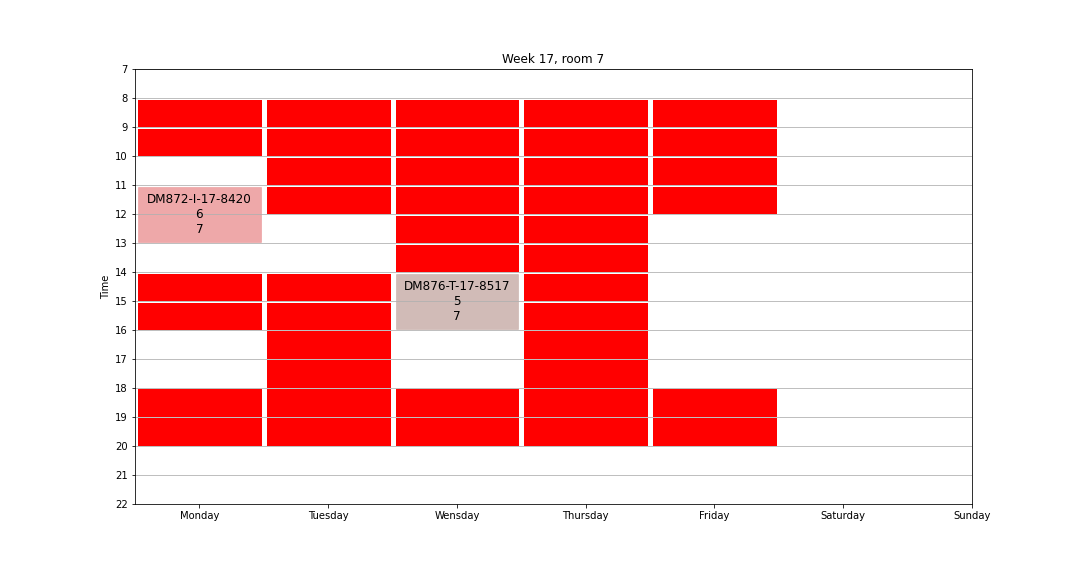
\includegraphics[scale=0.39]{../images/badslot.png}

    \subsection{}
    \begin{figure}
        \vspace{-3.2cm}
        \hspace*{-5cm}
        \begin{subfigure}{.85\textwidth}
            \centering
            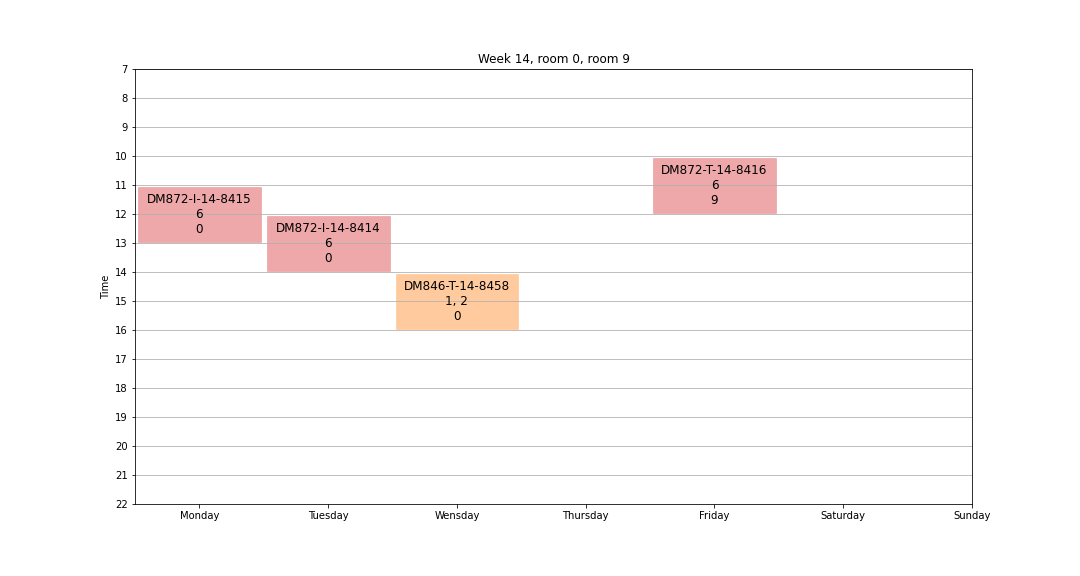
\includegraphics[width=1.1\linewidth]{../images/week-14.png}
        \end{subfigure}%
        \begin{subfigure}{.85\textwidth}
            \centering
            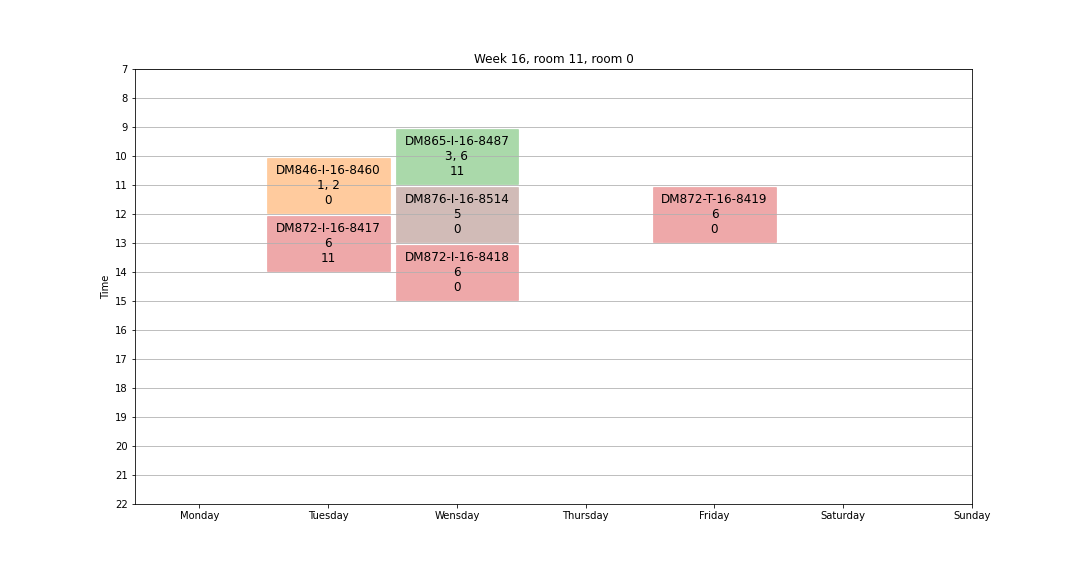
\includegraphics[width=1.1\linewidth]{../images/week-16.png}
        \end{subfigure}
        \hspace*{-5cm}
        \begin{subfigure}{.85\textwidth}
            \centering
            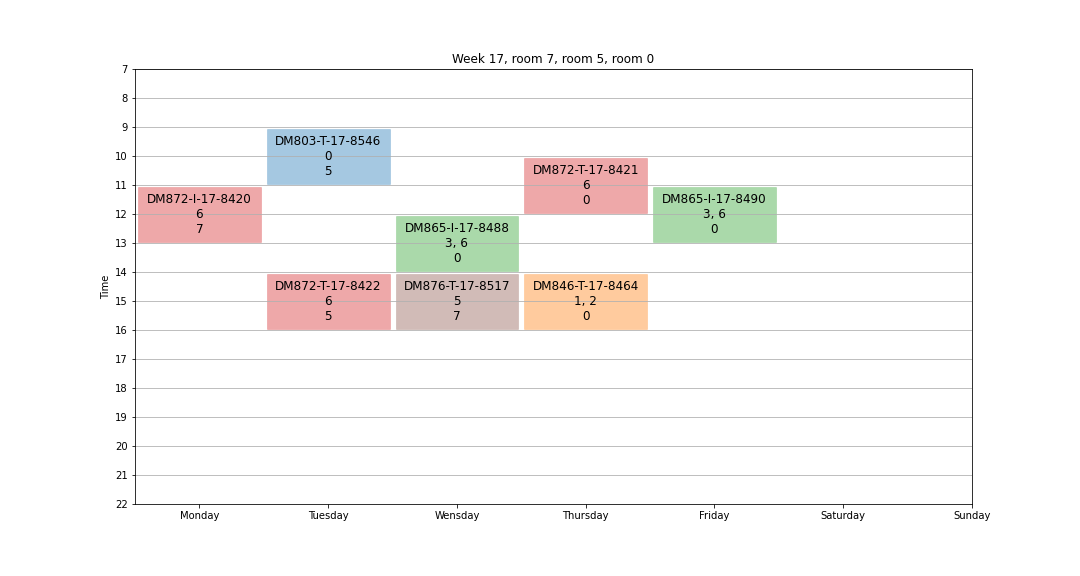
\includegraphics[width=1.1\linewidth]{../images/week-17.png}
        \end{subfigure}%
        \begin{subfigure}{.85\textwidth}
            \centering
            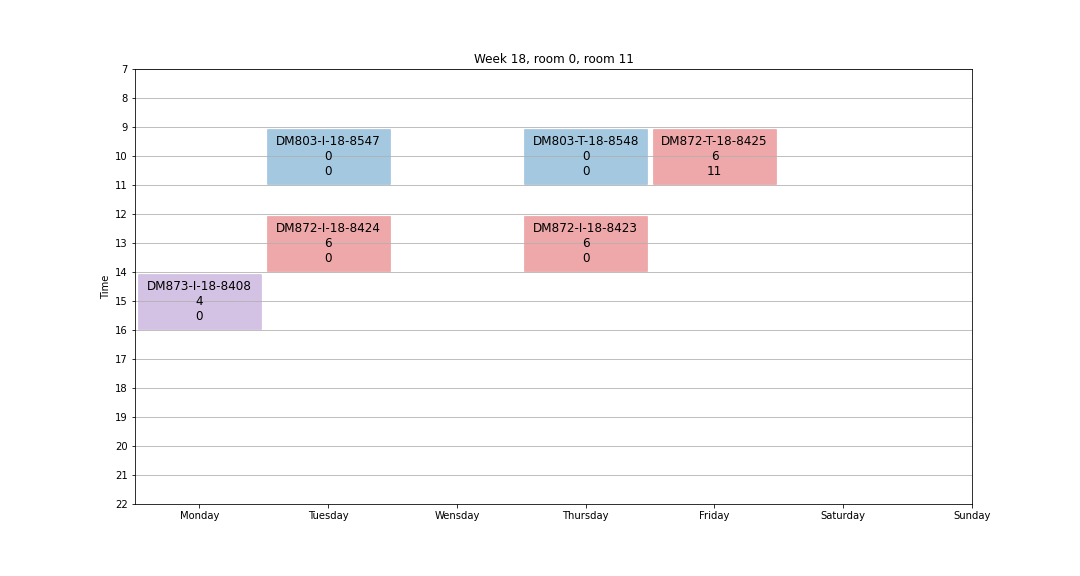
\includegraphics[width=1.1\linewidth]{../images/week-18.png}
        \end{subfigure}
        \hspace*{-5cm}
        \begin{subfigure}{.85\textwidth}
            \centering
            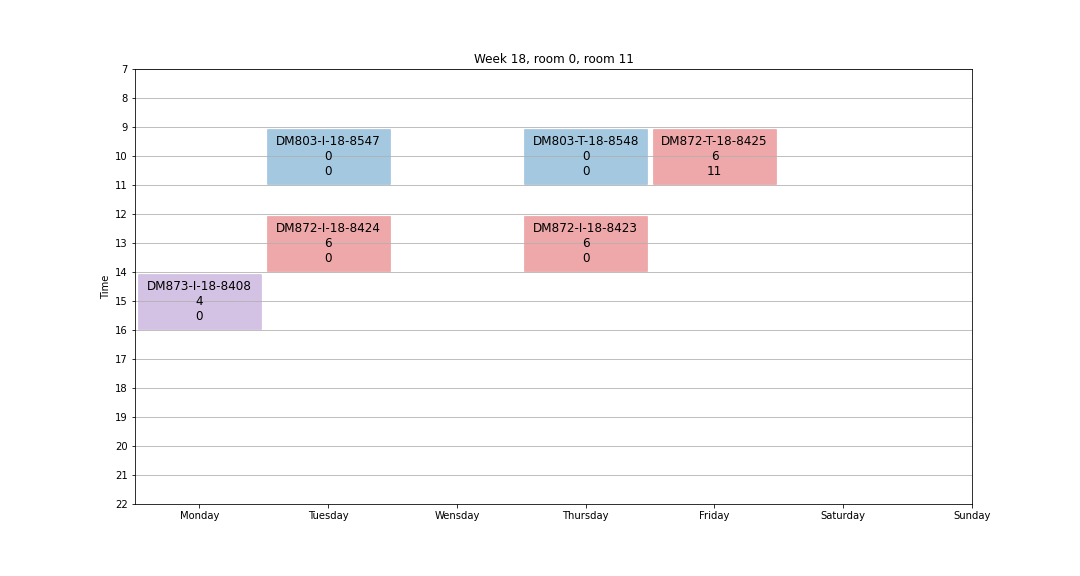
\includegraphics[width=1.1\linewidth]{../images/week-18.png}
        \end{subfigure}%
        \begin{subfigure}{.85\textwidth}
            \centering
            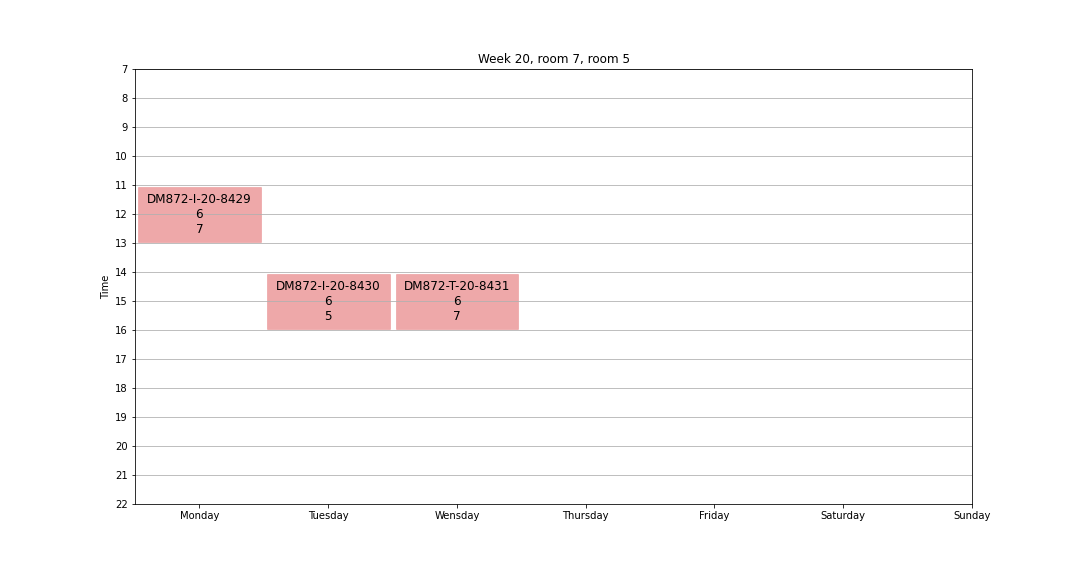
\includegraphics[width=1.1\linewidth]{../images/week-20.png}
        \end{subfigure}
        \hspace*{-5cm}
        \begin{subfigure}{.85\textwidth}
            \centering
            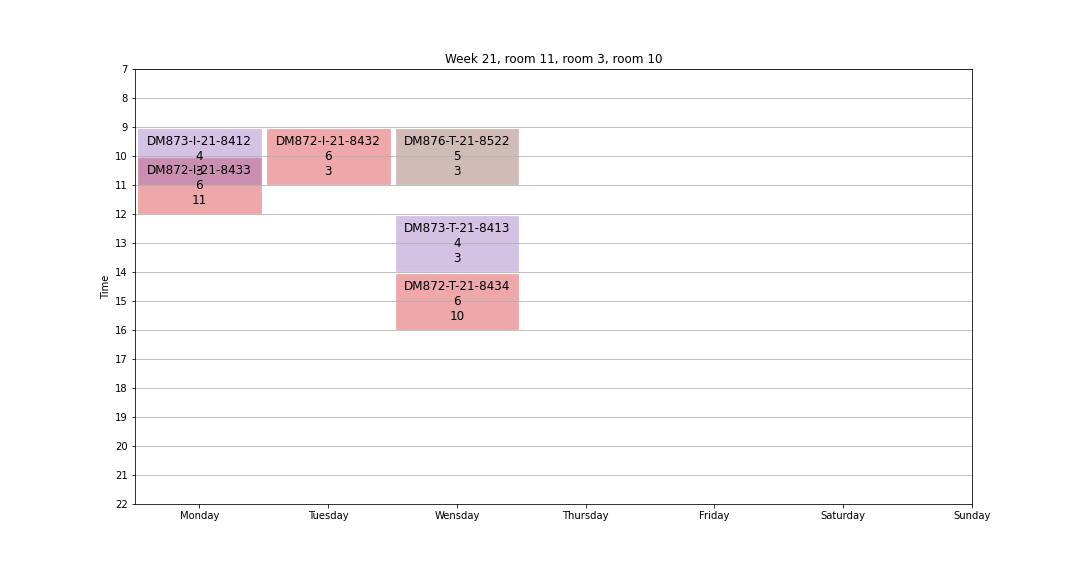
\includegraphics[width=1.1\linewidth]{../images/week-21.png}
        \end{subfigure}%
        \begin{subfigure}{.85\textwidth}
            \centering
            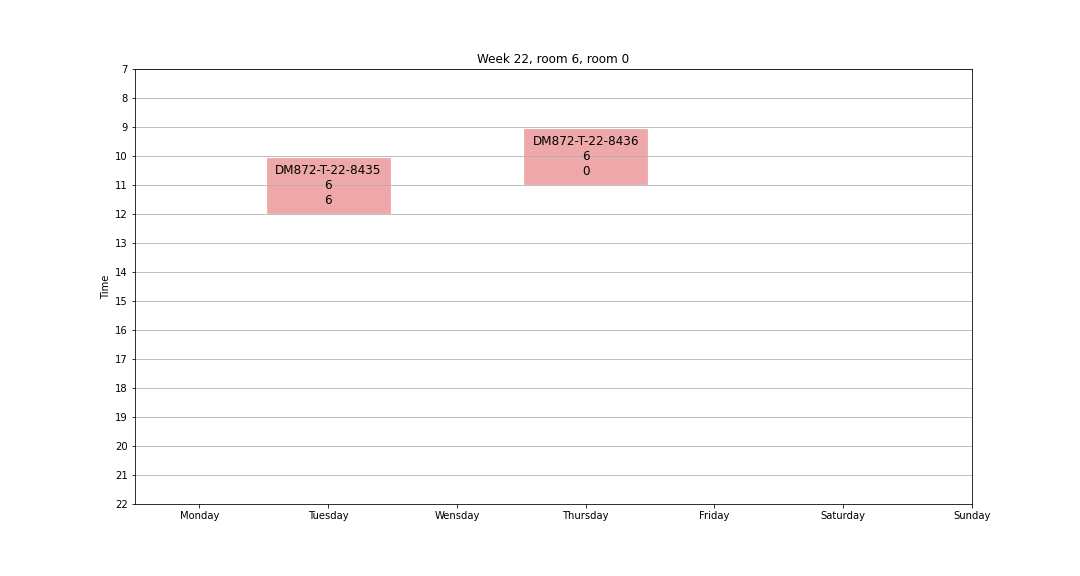
\includegraphics[width=1.1\linewidth]{../images/week-22.png}
        \end{subfigure}
    \end{figure}

    \clearpage
    \subsection{}
    \begin{lstlisting}[
        basicstyle=\tiny, %or \small or \footnotesize etc.
    ]
Academic license - for non-commercial use only
Read LP format model from file /tmp/tmpuxas4ygu.pyomo.lp
Reading time = 3.38 seconds
x2419281: 200802 rows, 2419281 columns, 9256086 nonzeros
Gurobi Optimizer version 9.0.2 build v9.0.2rc0 (linux64)
Optimize a model with 200802 rows, 2419281 columns and 9256086 nonzeros
Model fingerprint: 0x63bc928d
Variable types: 46 continuous, 2419235 integer (2419235 binary)
Coefficient statistics:
Matrix range     [1e+00, 2e+02]
Objective range  [1e+00, 1e+00]
Bounds range     [1e+00, 1e+00]
RHS range        [1e+00, 4e+00]
Presolve removed 194337 rows and 2389409 columns
Presolve time: 3.80s
Presolved: 6465 rows, 29872 columns, 286916 nonzeros
Variable types: 0 continuous, 29872 integer (29863 binary)

Root relaxation: objective -6.814444e+02, 2122 iterations, 0.07 seconds

Nodes       |    Current Node    |     Objective Bounds      |     Work
Expl Unexpl |  Obj  Depth IntInf | Incumbent    BestBd   Gap | It/Node Time

0     0 -681.44444    0  477          - -681.44444      -     -    4s
H    0     0                     303.0000000 -681.44444   325%     -    5s
H    0     0                     289.0000000 -681.44444   336%     -    7s
0     0 -592.41927    0  521  289.00000 -592.41927   305%     -    7s
H    0     0                     286.0000000 -592.41927   307%     -    7s
0     0 -541.64444    0  182  286.00000 -541.64444   289%     -    7s
0     0 -541.64444    0  146  286.00000 -541.64444   289%     -    7s
0     0 -541.64444    0  127  286.00000 -541.64444   289%     -    7s
0     0 -541.64444    0  127  286.00000 -541.64444   289%     -    7s
0     0 -541.64444    0  127  286.00000 -541.64444   289%     -    7s
0     0 -510.65735    0  178  286.00000 -510.65735   279%     -    8s
0     0 -483.73651    0  115  286.00000 -483.73651   269%     -    8s
0     0 -482.83814    0  115  286.00000 -482.83814   269%     -    8s
0     0 -482.79108    0  115  286.00000 -482.79108   269%     -    8s
0     0 -481.98580    0  119  286.00000 -481.98580   269%     -    8s
0     0 -481.38598    0  119  286.00000 -481.38598   268%     -    8s
0     0 -481.27077    0  111  286.00000 -481.27077   268%     -    8s
0     0 -481.27077    0  111  286.00000 -481.27077   268%     -    8s
0     0 -406.84444    0  179  286.00000 -406.84444   242%     -    9s
0     0 -406.64444    0  169  286.00000 -406.64444   242%     -    9s
0     0 -406.64444    0  182  286.00000 -406.64444   242%     -    9s
0     0 -379.77425    0  154  286.00000 -379.77425   233%     -    9s
H    0     0                     284.0000000 -379.77425   234%     -   10s
H    0     0                     282.0000000 -379.77425   235%     -   10s
0     0 -379.77425    0  167  282.00000 -379.77425   235%     -   10s
0     0 -379.73375    0  198  282.00000 -379.73375   235%     -   10s
0     0 -379.73375    0   65  282.00000 -379.73375   235%     -   10s
0     0 -379.73375    0   57  282.00000 -379.73375   235%     -   11s
0     2 -379.73375    0   48  282.00000 -379.73375   235%     -   12s
77    51  -31.94821   11  132  282.00000 -379.73375   235%   255   15s
H   78    51                     281.0000000 -379.73375   235%   252   15s
753   552  155.00000   74   60  281.00000 -379.73375   235%   127   20s
1101   857  196.00000   97   45  281.00000 -379.73375   235%  96.4   25s
1491  1084  195.00000  139  420  281.00000 -377.27831   234%  94.4   30s
1503  1092  199.00000   77   38  281.00000 -102.34637   136%  93.6   35s
1506  1094  153.00000   81   84  281.00000 -101.24655   136%  93.4   40s
1510  1097  199.00000   75   39  281.00000 -101.24655   136%  93.2   48s
1520  1099  184.87256   15  132  281.00000 -101.24655   136%   112   50s
1537  1109  216.67776   18  206  281.00000 -101.24655   136%   116   56s
1603  1137  239.02273   23  185  281.00000 -101.24655   136%   128   60s
1958  1242  246.00000   47  115  281.00000 -101.24655   136%   145   65s
2181  1279  197.41566   33  222  281.00000    4.36059  98.4%   156   70s
2298  1301  133.73087   24  235  281.00000    6.89482  97.5%   162   75s
2664  1386  222.95477   34  207  281.00000  137.92439  50.9%   178   80s
3017  1459  218.56127   33  221  281.00000  153.44751  45.4%   189   85s
3280  1522  251.36274   31  163  281.00000  163.08980  42.0%   196   90s
3620  1561  252.00000   36   54  281.00000  165.29173  41.2%   200   97s
3874  1634  258.04762   34  246  281.00000  165.29173  41.2%   205  101s
4106  1623  212.95991   24  188  281.00000  167.75962  40.3%   206  105s
4474  1649  231.04545   34  152  281.00000  176.09166  37.3%   210  111s
4909  1720  261.08333   33  203  281.00000  180.67085  35.7%   213  122s
5062  1761  222.45925   31  202  281.00000  184.09907  34.5%   214  125s
5609  1923     cutoff   38       281.00000  188.23989  33.0%   215  131s
6023  2024  260.05147   32  178  281.00000  189.36172  32.6%   212  136s
6458  2147  261.08333   32  135  281.00000  190.49172  32.2%   211  141s
6897  2285  261.32868   38  164  281.00000  192.42899  31.5%   210  146s
7412  2435  255.04545   32  209  281.00000  194.53652  30.8%   208  151s
7704  2472  257.08333   35  157  281.00000  198.23841  29.5%   207  155s
8312  2625  239.02347   35  194  281.00000  200.51009  28.6%   203  161s
8625  2718  237.02013   32  172  281.00000  202.43727  28.0%   201  165s
9282  2871  259.71231   38  171  281.00000  205.39304  26.9%   198  172s
9610  2952     cutoff   43       281.00000  206.87891  26.4%   197  175s
10399  3058  260.33031   29  189  281.00000  211.12053  24.9%   192  183s
10822  3085  261.32868   39  175  281.00000  213.43063  24.0%   191  190s
11643  3191  246.23320   22  178  281.00000  216.31443  23.0%   187  198s
12126  3211  264.61771   46  176  281.00000  217.44236  22.6%   184  201s
12639  3235  268.50893   30  161  281.00000  219.51989  21.9%   181  206s
13750  3221  243.04861   30  180  281.00000  226.04217  19.6%   177  218s
14185  3214  260.34989   35  216  281.00000  228.28803  18.8%   176  222s
14796  3207     cutoff   43       281.00000  231.15008  17.7%   175  238s
15058  3208  261.32868   39  225  281.00000  232.04545  17.4%   174  242s
15731  3184  268.17560   30   24  281.00000  233.04545  17.1%   171  247s
16450  3146  264.11552   31  203  281.00000  234.01935  16.7%   168  252s
17168  3051  270.04762   32  182  281.00000  235.04762  16.4%   166  257s
17892  2943     cutoff   33       281.00000  237.12314  15.6%   162  262s
18583  2774     cutoff   32       281.00000  238.76478  15.0%   159  267s
19312  2595     cutoff   33       281.00000  241.00000  14.2%   155  273s
20152  2370  267.00000   36   19  281.00000  244.00000  13.2%   152  278s
21065  2029     cutoff   43       281.00000  246.04544  12.4%   149  286s
22056  1632  266.04545   30  137  281.00000  251.00000  10.7%   144  291s
22955  1243 infeasible   41       281.00000  258.00000  8.19%   141  297s
23925   749     cutoff   40       281.00000  260.00000  7.47%   136  302s
24765   209  267.01684   36  217  281.00000  262.01684  6.76%   133  306s

Cutting planes:
Gomory: 41
Projected implied bound: 2
Clique: 2
MIR: 18
Flow cover: 48
GUB cover: 8
Inf proof: 18
Zero half: 30
RLT: 14

Explored 25761 nodes (3329380 simplex iterations) in 307.73 seconds
Thread count was 16 (of 16 available processors)

Solution count 6: 281 282 284 ... 303

Optimal solution found (tolerance 1.00e-04)
Best objective 2.810000000000e+02, best bound 2.810000000000e+02, gap 0.0000%
    \end{lstlisting}

\end{document}